% This is the template for submission of abstracts to NetSci 2017 in Indianapolis, IN.
% It is modified from NetSci 2016.
% The editor of the booklet reserves the right to modify your submission.

%% To process this file run LaTeX2e

%%********DO NOT EDIT****************
\documentclass[12pt]{article}
\usepackage{mathptmx}
\usepackage{graphicx}
\pagestyle{empty}

\setlength\topmargin{0pt}
\addtolength\topmargin{-\headheight}
\addtolength\topmargin{-\headsep}
\setlength\oddsidemargin{0pt}
\setlength\textwidth{\paperwidth}
\addtolength\textwidth{-2in}
\setlength\textheight{\paperheight}
\addtolength\textheight{-2in}
\usepackage{layout}

\renewcommand{\title}[1]{\noindent\textbf{#1}\bigskip\\}
\renewcommand{\author}[1]{\noindent #1\bigskip\\}
%%***********************************

\begin{document}

%**********USER DEFINED**************
%Enter title here
\title{Towards Attack-Tolerant Networks: Multipath Fault Tolerance}
%Enter author(s) and address here
\author{Edward L. Platt$^1$ and Daniel M. Romero$^1$\bigskip\\
{\small
1. University of Michigan, Ann Arbor, MI, USA\\
}
}
%Enter abstract here
Networks with single points of failure are particularly susceptible to
targeted attacks.
In communication networks, these types of faults can leave users vulnerable to
censorship and targeted surveillance,
even when cryptography is utilized.
Centralized networks have single points of failure by definition,
leading to a growing popularity in decentralized architectures and protocols.
However, centralized network structure can arise even when protocols are
decentralized.
Despite being based on decentralized protocols,
the Internet and World-Wide Web have
been shown both theoretically and historically to be highly susceptible to
adversarial faults [1], in part due to emergent structural centralization.
Existing network trust models, such as webs of trust [2], fail to adequately address
network structure.
We describe a novel, adversarial fault-tolerant,
concurrent multipath routing algorithm for the decentralized
butterfly network topology [3].
We also develop a partial trust model that makes it possible to
quantify the adversarial fault tolerance of a network,
and which makes more realistic transitivity assumptions than webs of trust.
When network topology can be dictated, these results can be used to create
scalable, attack-tolerant infrastructures. More generally, our results provide
a formalism for evaluating the effects of network structure on adversarial
fault tolerance.

\bigskip
\noindent[1] R. Albert et al. Error and attack tolerance of complex networks. {\em Nature,} 406(6794), 2000.
\\
\noindent[2] P. R. Zimmermann. {\em The Official PGP User's Guide.} MIT Press, 1995.
\\
\noindent[3] A. D. Kshemkalyani and M. Singhal. {\em Distributed Computing: Principles, Algorithms, and Systems}. Cambridge University Press, 2008.
\\

\begin{figure}[!h]
\begin{center}
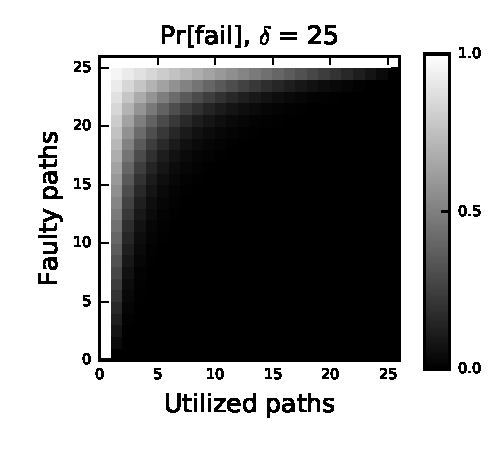
\includegraphics[scale=0.75]{fig-perror}
\end{center}
\caption{
In multipath fault tolerance,
the failure probability decreases rapidly with the number of
message copies, and increases slowly with the number of faults.
Messages are difficult to attack and easy to defend.
}
\end{figure}
% Place the abstract of your talk/poster here, 250 Words maximum.
% Mathematical formulae may be set in LaTeX, but do NOT use the
% bibliography environment -- if you must have references, use an 
% enumerated list.
%
% Your abstract (plus one figure) should not exceed one page.
%
% Check carefully.

%************************************
\end{document}